\documentclass[11pt]{article}
\usepackage{setspace}
\setstretch{1}
\usepackage{amsmath,amssymb, amsthm}
\usepackage{graphicx}
\usepackage{bm}
\usepackage[hang, flushmargin]{footmisc}
\usepackage[colorlinks=true]{hyperref}
\usepackage[nameinlink]{cleveref}
\usepackage{footnotebackref}
\usepackage{url}
\usepackage{listings}
\usepackage[most]{tcolorbox}
\usepackage{inconsolata}
\usepackage[papersize={8.5in,11in}, margin=1in]{geometry}
\usepackage{float}
\usepackage{caption}
\usepackage{esint}
\usepackage{url}
\usepackage{enumitem}
\usepackage{subfig}
\usepackage{wasysym}
\newcommand{\ilc}{\texttt}
\usepackage{etoolbox}
\usepackage{algorithm}
\usepackage{changepage}
% \usepackage{algorithmic}
\usepackage[noend]{algpseudocode}
\usepackage{tikz}
\usetikzlibrary{matrix,positioning,arrows.meta,arrows}
\patchcmd{\thebibliography}{\section*{\refname}}{}{}{}
% \PassOptionsToPackage{hyphens}{url}\usepackage{hyperref}

\providecommand{\myceil}[1]{\left \lceil #1 \right \rceil }
\providecommand{\myfloor}[1]{\left \lfloor #1 \right \rfloor }


\begin{document}



\title{\textbf{CSDS 455: Homework 12}}

\author{Shaochen (Henry) ZHONG, \ilc{sxz517}}
\date{Due and submitted on 10/05/2020 \\ Fall 2020, Dr. Connamacher}
\maketitle


\section*{Problem 1}

Assume we have graph $G'$ which is identical with $G$, but already colored by $\chi(G)$ colors. We may have a vertex ording of $v_1, v_2, ..., v_n$ (assume $|V(G)| = n$), where $v_1$ to $v_i$ have color $c_1$, $v_{i+1}$ to $v_{j}$ have color $c_2$, ..., and $v_k$ to $v_n$ have color $c_{\chi(G)}$ (for $i < j < k < n$).

This votex odering will guarteen a $\chi(G)$-coloring of $G$. As if the a vertex $v$ has a color of $c$ in $G'$, then the next vertex $v'$ from the above ordering will either have the same color as $v$ in $G'$, in this case the greedy algorithm will color $v'$ the same color as $v$; or it will have a different color, in this case the greedy algorithm will try all ``used'' colors\footnote{Colors used on vertices before $v'$ in the listed ordering} -- which obviously not going to work as $G'$ represents the minimum colored graph of $G$ -- then the algorithm will give $v'$ a new color. Following this order the algorithm will color $G$ just as $G'$, which contains $\chi(G)$ colors.


\section*{Problem 2}

Let $G$ being a bipartite graph, where each of its part partision has $n$ vertices (so $2n$ vertices in total). We denote the vertices in partition $U$ to be $u_1, u_2, ..., u_n$, and likewise for vertices in partition $V$.

For a vertex $u_i \in V(U)$, we connect it to all vertices in $U$ except to $v_i$; we do the same to all vertices in $U$. The order that produce a $2n$-coloring of $G$ would be $u_1, v_1, u_2, v_2, ..., u_n, v_n$.

It is because if a $u$ vertex and its next $v$ vertex have the same subscript, they will not be connect and the greedy algorithm may assign the same color to them. However, if a $v$ vertex and its next $u$ vertex have the different subscripts (specifically, $v_i$ and $u_j$ where $j = i+1$), the $u$ vertex will be connected too all currently colored $v$ vertices, this means the greedy algorithm will have to assign a new color for it. Since we have $n$ pairs of neighbor $(v_i, u_j)$ where $j = i+1$, $n$ new colors are were assigned and the a $n$-coloring of $G$ is obtained.


\section*{Problem 3}

We first want to show for any $k$-chromatic graph has a $k$-critical subgraph: For any given $k$-chromatic graph $G$, if it is a critical $k$-critical graph by itself, then we are done. If $G$ itself is not a $k$-critical graph, then there must be a $v \in V{G}$ where $\chi(G-v) \geq \chi(G)$. Since removing a vertex will not increase the minimum coloring of a graph, for this vertex we must have $\chi(G-v) = \chi(G)$. If the new $G$ (with $v$ removed) is still not $k$-critical, we will remove another $v$ where $\chi(G-v) = \chi(G)$, untill we have a $k$-critical subgraph out of $G$.\newline

We will then show every vertex in $k$-critical graph $G'$ has a minimum degree of $k-1$. Assume there is $v \in V(G')$ where $d(v) = k-2$. Due to the property of being a $k$-critical graph, we must have $\chi(G'-v) <= k - 1$. Since $x$ has only $k-2$ neighbors, we may always color $x$ in $G'$ with the $k-1$-th color used in $G' - v$. This suggests $G'$ is $k-1$ colorable in stead of $k$, which is contradiction to the setup of $G'$. Thus, if $G'$ is $k$-critical, $\delta(G') \geq k - 1$.


\section*{Problem 4}

We will introduce a way to construct graph $G$ that fits the question requirements. We first draw a vertex $X$, then we draw $\Delta(G)$ number of vertices (we denotes them alphabetically). In the base case of $\Delta(G) = 4$, we may have the following graph for fundation.

\begin{figure}[H]
    \centering
    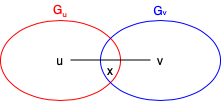
\includegraphics[width=0.2\linewidth]{{fig/fig_p4_1.png}}
\end{figure}

We will notice between the first and last alphabetically named vertices, there will be $\Delta(G) - 2$ vertices in between (non-inclusive), we call the path between them as $P$. We then remove the first and last vertices of $P$ to make $P'$, and connect the $V(P')$ to $X$. In this case, $P$ will be $B, C$; and since $P$ has only 2 vertices, we have $|V(P')| = 0$, thus nothing from $P'$ conncted to $X$.

We then try to draw 3 $\Delta(G)-2$ cliques among the alphabetically named vertices. In this case it will be:

\begin{gather*}
    A \ B \\
    B \ C \\
    C \ D
\end{gather*}

Where $AB$, $BC$, $CD$ each formed a 2-clique. We may tell there must be $\chi(G) = 3$. As the second $\Delta(G)-2$-clique ($B \ C$) must use 2 colors, then $A$ and $D$ must have a different color, this make $X$ must have the 3-rd color; thus accomplishes $\chi(G) = 3$ and satisfies the $\chi(G) \geq \Delta(G) - 1$ requirement.

We also know that this graph does not contain any $\Delta(G) - 1$ clique as each two rows of clique will have at least 1 different vertex.

We also know that this graph will not be have a maximum degree $\geq 4$, as there are only 5 vertices in it. Actually, to make $\Delta(G) = 4$, we must place some dummy vertices connected to $X$ (which won't affect the $\chi(G)$). The below graph is a solution to $\Delta(G) = 4$.


\begin{figure}[H]
    \centering
    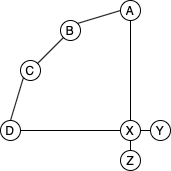
\includegraphics[width=0.2\linewidth]{{fig/fig_p4_2.png}}
\end{figure}

Since $\Delta(G) = 4$ has no $P'$, here is $\Delta(G) = 5$ to help demonstrating the idea (in this case $P'$ is $C$):

\begin{figure}[H]
    \centering
    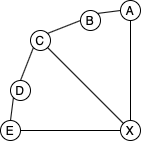
\includegraphics[width=0.2\linewidth]{{fig/fig_p4_3.png}}
\end{figure}

Which will have $\Delta(G) - 2= 3$-cliques on:

\begin{gather*}
    A \ B \ C \\
    B \ C \ D \\
    C \ D \ E
\end{gather*}

Where $B \ C \ D$ willl use up 3 color, and $A, E$ (for the sake of having minimum coloring), must use the color of $D, B$. However, since $A, E, C$ are all connected to $X$, $X$ must have the 4-th color, making $\chi(G) = 4$. The graph has $6$ vertices so we can at most $\Delta(G) = 5$; we may always have $\Delta(G) = 5$ by adding dummy vertices, although it is not necessary at this case since $d(C) = 5$. And the graph conyains no $\Delta(G) - 1 = 4$ cliques as each two rows of clique will have at least 1 different vertex.\newline



Now we like to show this method also works for $\Delta(G) = k$. We may first have $X$ and $k$ alphabetically named vertices, all connected as a cycle. We then identify the $P'$ and connect all $V(P')$ to $X$. We then form 3 $\Delta(G) - 2$-cliques on the alphabetically named vertices, which will be like (Note $k$ means the $k-th$ alphabetically named vertex):

\begin{align*}
    A \ B \ C \ D \ E \ ... \ &k - 2\\
    B \ C \ D \ E \ F \ ... \ &k - 1 \\
    C \ D \ E \ F \ G \ ... \ &k
\end{align*}

We know that the second row of clique will use up $k - 2$ colors and $A, k$ won't share a color. We also know that $k - 4$ vertices ($\in V(P')$) will be connected to $X$ along with $A$ and $k$, where all of them have different colors. This suggest $X$ must have the $k-1$-th color.\newline

We have showed $\chi(G) = k-1$. We now this $G$ contains no $k-1$ cliques as every 2 rows of $k-2$-cliques have at least 1 vertex differ. We also know that this graph will not have a maximum degree $\geq k$, as it has only $k+1$ vertices.

We have showed this graph constructing method works for any arbitary $G$ with $\Delta(G) \geq 4$.

% \section{References}
%
% \nocite{*}
% \raggedright
% \bibliography{references.bib}
% \bibliographystyle{plain}


\end{document}